
%% 
%% Copyright 2007-2020 Elsevier Ltd
%% 
%% This file is part of the 'Elsarticle Bundle'.
%% ---------------------------------------------
%\documentclass[preprint,12pt]{elsarticle}
% \documentclass[review,12pt, 3p, times]{elsarticle}
\documentclass[preprint,11pt,3p]{elsarticle}
\usepackage{amssymb}
\usepackage{graphicx}
\usepackage{longtable}
\usepackage{tipa}
\usepackage{cancel}
\usepackage{ulem}
\usepackage{pgf}
\usepackage{silence}
\usepackage{amssymb}
\usepackage{lineno}
\usepackage{enumitem}
\usepackage{lineno,hyperref}
\usepackage{natbib,stfloats}
\usepackage{multirow}
\usepackage{array}
\usepackage{multicol}
\usepackage{booktabs}
\usepackage{mathrsfs}
\usepackage{graphicx}
\usepackage{epstopdf}
\usepackage{latexsym}
\usepackage{mathtools}
\usepackage{algorithm}
\usepackage{algorithmic}
\usepackage{amsmath,amsfonts,amssymb}
\usepackage{rotating}
\usepackage{color}
\usepackage{colortbl}
\usepackage[caption=false]{subfig}
\usepackage[ruled,vlined,algo2e]{algorithm2e}
\usepackage{setspace}
\usepackage{tabularx}
\usepackage{xcolor}
\usepackage{adjustbox}
\usepackage{tikz}

\usepackage{cancel}
\hypersetup{colorlinks,linkcolor={blue},citecolor={blue},urlcolor={red}} 

\usepackage{setspace}
\usepackage{lineno}
\usepackage{amssymb}
\usepackage{pifont}
\usepackage{svg}
\usepackage{tikz,lipsum,lmodern}
\usepackage[most]{tcolorbox}
\usepackage{pdfpages}

% \definecolor{my-blue}{cmyk}{0.80, 0.13, 0.14, 0.04, 1.00}
\definecolor{q_color1}{HTML}{F0F8FF}
\definecolor{q_color2}{HTML}{91A3B0}

\definecolor{r_color1}{HTML}{d9dbde}
\definecolor{r_color2}{HTML}{737475}

\newcounter{magicrownumbers}
\newcommand\rownumber{\stepcounter{magicrownumbers}\arabic{magicrownumbers}}
\newcommand{\cmark}{\ding{51}}%
\newcommand{\xmark}{\ding{55}}%


\journal{journal of Computers and Industrial Engineering}

\begin{document}
\begin{center}
	\begin{huge}  
		\textbf{ \quad \quad Response to reviewers}
	\end{huge}  
	\newline
	\newline
	\textbf{Ms. Ref. No.: PROECO-D-23-01945}
			
	\textbf{Title: "Incorporating Uncertain Human Behaviour in Production Scheduling for Enhanced Productivity in Industry 5.0 context" } 
 \newline
 International Journal of Production Economics 
	
\end{center}

First of all, we would like to thank all the reviewers for the thorough revision and valuable comments on the previous version. We have carefully read and analyzed each one of your comments, and we took them into consideration in preparing this new version. We hope that this new version is now much clearer. In the following, we explain our interpretation of your comments and the way in which we took into account each one. In addition, the paragraphs containing modifications have been highlighted in the text (in blue). We have also linked each comment to the corresponding point in the manuscript using the notation "$[id]Rn^{q}$", where "n" represents the reviewer number, "q" represents the comment number, and "id" is the comment identifier. This notation makes it easy to find and track the reviewer's feedback.





\newpage 
% Thank you for the relevant remark, 
Thank you for taking the time to provide detailed feedback on our manuscript. We sincerely appreciate your thorough review and insightful comments. Your constructive criticism and valuable suggestions will undoubtedly contribute to enhancing the quality and clarity of our work. We have carefully considered each of your points, and we would like to address them accordingly.
\section{Reviewer 1: }
This paper investigates the impact of workers' individual behavior on the productivity of the industrial system. To do so, Markov chain was adopted to represent worker's productive and non-productive states and simulation and non-linear mathematical model were used to determine the impact that different workers' profile can have on final throughput of a flow-shop production system.

I personally believe that introducing the behaviors of workers inside mathematical modelling to predict the final output of a system is fundamental but still very challenging. Human behaviors is very difficult to be predicted, differently from other human features that can be almost directly quantified, such as the accumulated fatigue of workers (e.g., through the adoption of some heart rate or breathing rate sensors, or biosensors based on the sweating level of the skin) .

I think this contribution can be considered as a step further in the direction of take into account personal behaviors in mathematical models of the most challenging scheduling problems, however, I want to share with the authors some of the major concerns I had while reading this work, which, in my personal opinion, lacks of scientific rigorousness in the experimental test and, in particular, in the determination of profile matrix values. I hope my comments can help authors to improve the quality of their work.

\begin{tcolorbox}[colback=q_color1,colframe=q_color2,title=Q1 :]	
	Industry 5.0 concept can be better addressed. This term was forged by the European Commission and the difference from the Industry 4.0 for what concern the central role of human being can be better explain. In particular, more than sustainability and resilience pillars of the paradigm, authors may focus on the social sustainability and on the workforce development to create a resilient workforce.
\end{tcolorbox}
   

\begin{tcolorbox}[colback=r_color1,colframe=r_color2,title=Response Q1 :]
	Thank you for the relevant remark, we improved the paragraph talking about industry 5.0 and social sustainability by introducing new references talking about this concept (c.f. page 3). 
	% 
	% je pense qu'ilfaut rajouter un paragraph dans l'introduction sur le social sustainability.
	% \begin{itemize}
	% \item \cite{trost2022social}
	% \item La durabilité sociale est un concept complexe qui englobe un large éventail de dimensions, notamment la cohésion sociale, l'équité, la justice sociale, la protection des droits fondamentaux et la participation démocratique. 
	% \item la durabilité sociale est "la capacité d'une société à se maintenir et à se développer dans le temps tout en préservant les conditions sociales, économiques et environnementales nécessaires pour assurer le bien-être des générations présentes et futures".
	%  Exemples concrets de durabilité sociale
	% 	\item Exemples concrets de durabilité sociale 
	% 	      \begin{itemize}
	% 	      	\item La réduction des inégalités de revenus et de patrimoine
	% 	      	\item L'amélioration de l'accès à l'éducation, à la santé et au logement
	% 	      	\item La promotion de la diversité et de l'inclusion
	% 	      	\item Discrimination et violence selon que vous êtes un homme ou une femme
	% 	      	\item La protection des droits des enfants, des personnes handicapées et des personnes âgées
	% 	      	\item La promotion de la participation citoyenne et de la démocratie
			      	          
	% 	      \end{itemize}
			      
	% 	\item Défis de la durabilité sociale
	% 	      \begin{itemize}
	% 	      	\item La mondialisation et ses impacts sur les marchés du travail et les systèmes de protection sociale
	% 	      	\item Les changements démographiques et le vieillissement de la population
	% 	      	\item Les crises économiques et leurs conséquences sociales
	% 	      	\item L' montée des inégalités et des tensions sociales
	% 	      	\item Les défis liés à la migration et à l'intégration
	% 	      \end{itemize}
	% 	\item Importance de la durabilité sociale :
			      
	% 	      La durabilité sociale est essentielle pour assurer le bien-être des individus et des communautés, et pour créer des sociétés justes, équitables et prospères. Une société durable est une société qui est capable de répondre aux besoins de ses membres aujourd'hui, sans compromettre la capacité des générations futures à répondre aux leurs.
			      
			      
			      
			      
			      
			      
	% \end{itemize}
			
		
			
\end{tcolorbox}
\begin{tcolorbox}[colback=q_color1,colframe=q_color2,title=Q2  :]	
	In the literature review, authors considered some works related to the prediction of customers' behaviors to investigate the methods adopted in comparison to the ones that could be applied to the industrial work field. Nevertheless, authors did not extensively proposed any comparison between the model they developed and the ones they found on customers' behaviors prediction. This research topic should be at least discussed more if authors want to report some parallelism on this direction.
\end{tcolorbox}


\begin{tcolorbox}[colback=r_color1,colframe=r_color2,title=Response Q2  :]
	Thank you for this insightful observation. We recognise that a comparison between the model we developed and existing models for customer behaviour prediction is not clearly highlighted. The main difference between these models and the one we developed is the time scale and the type of behaviour modelled. Therefore, we added more explanation about the modelling principles of the cited customer behaviors prediction models in order to understand their similarities with our model (c.f. Page 6). 
	    
	%ERG theory (Existence, Relatedness, Growth), proposed in 1969  by Alderfer, puts emphasis on the needs of individuals in a hierarchical order. The acronym ERG stands for existence, relatedness, and growth. This theory is based on Maslow's work, which reduced the number of needs to three. However, ERG theory differs from Maslow's in three ways: (1) it allows for multiple levels to be pursued at the same time; (2) it allows for different orders of needs for different people; and (3) if the highest level of needs remain unsatisfied, a person may regress to a lower level of needs that are more easily fulfilled.
			
	%\citep{chang2008synthesized} used the Markov chain to modeling customer profiles, with the hierarchy of needs represented by states. In this context, the different states of the Markov chain correspond to different levels or categories of customer needs. The transition probabilities between states reflect the likelihood of customers moving from one need category to another over time. By analyzing observed transitions and estimating transition probabilities, the Markov chain model can provide information on customer behavior and the dynamics of their needs.
\end{tcolorbox}
\begin{tcolorbox}[colback=q_color1,colframe=q_color2,title=Q3  :]	
	At page 5, authors state the following sentence "Although the human being has often been taken into account in the various operations management models in the literature, especially regarding his unpredictable behavior, his fatigue, and his performance in performing tasks, we did not find any research work that takes into account the fact that human behavior and performance can change from one worker to another." I think this sentence is misleading since authors stated that unpredictable behavior together with fatigue have already been considered in mathematical model, however, authors in the abstract stated that human behavior is almost always neglected. Hence, what it is not very clear to me is if "human unpredictable behavior" has already been considered in literature (such as the sentence I reported in this comment states) or is it something completely new that authors want to include in this mathematical model?
\end{tcolorbox}


\begin{tcolorbox}[colback=r_color1,colframe=r_color2,title=Response Q3  :]
	We agree with the reviewer that the mentioned sentence is quite confusing. 	
	In fact, we meant that in existing literature, while certain aspects of human behavior like unpredictability and fatigue have been acknowledged in operations management models, they're typically treated as general attributes without distinguishing between individual worker profiles. The sentence you've highlighted aims to emphasize the lack of specific research considering variations in human behavior and performance among different workers within these models. The intent is not to suggest that unpredictability itself hasn't been addressed at all, but rather that the differentiation between individual variations in behavior and performance across workers remains largely unexplored within the existing mathematical frameworks.
	    
	We modified the paragraph that you mentionned  and the abstract in order to make it more clear and making the difference between our contribution and the existing works (c.f. Page 7 and abstarct).  
\end{tcolorbox}
\begin{tcolorbox}[colback=q_color1,colframe=q_color2,title=Q4  :]	
	  At page 6, authors report the "worker profile composition" but the lack of clear explanation of how a worker's profile is composed can create confusion to the readers. Hence, I suggest authors to anticipate the explanations of what are productive and non-productive zones.
\end{tcolorbox}

\begin{tcolorbox}[colback=r_color1,colframe=r_color2,title=Response Q4 :]
	% il faut remonter l'explication des types de zones. 
	Thank you for this suggestion to anticipate the explanation of productive and non-productive zones. 
	Therefore, we added a paragraph (c.f. Page 7) that explains the concept of worker profile and its associated framework.
	% These worker profiles are defined by their punctuality with Markov chain model ,Note that state of Markov chain  represented by (Productive zones or non-productive zones). Productive zones denote areas where workers actively contribute to production, while non-productive zones represent phases where their contribution is absent. 
	% We added a paragraph 
			
	
	% Q5: The worker profile composition is based on a single attribute, the transition between  zones -punctuality-, which is modeled by a Markov chain and utilized in a simulation.
		
	%Q5: Different and diverse behavioral profiles of workers are affected by various factors (such as fatigue, experience,  age, etc.), which we have tried to translate into a model determining machine availability and unavailability. These models have been integrated into the optimization model.
		
	%Q8: The variability of NPZ lies in the probability of staying, which affects the length of stay. In fact, the probability of NPZ varies from person to person. For example, in the area of sming, there are individuals who don't sme, others who sme occasionally and others who sme a lot, representing the proportion of departures and stays within the NPZ (sming zone), ditto for the other zones. We have not taken into account the most attractive and influential zones. This varies from person to person and "is reflected in the profile or probability of transition between NPZs and the probability of staying there. Thanks for the important observations, which could be an addition in future work.
					
\end{tcolorbox}
\begin{tcolorbox}[colback=q_color1,colframe=q_color2,title=Q5  :]	
	Which is the difference between "worker profile composition" and "various heterogeneous behavioral profile of workers"?
	 
\end{tcolorbox}


\begin{tcolorbox}[colback=r_color1,colframe=r_color2,title=Response Q5  :]
	Actually, there is a slight difference between the meaning of ``worker profile composition'' and ``various heterogeneous behavioural profiles of workers''. What we meant by the first expression is the fact of testing different scenarios representing different configurations of homogeneous and heterogeneous sets of workers regarding their behavioural profiles.
	
	
	
	
	% We have made adjustments to avoid any confusion in meaning Between model of the worker profile and various heterogeneous behavioral
	
	% 1-the composition of  the worker profile
	% 2-considers various heterogeneous behavioral profiles of workers.
	% 11- the composition of behaviour profiles (homogeneous and heterogeneous) of workers
	  
\end{tcolorbox}
\begin{tcolorbox}[colback=q_color1,colframe=q_color2,title=Q6  :]	
	At page 6, authors state that this work deals with dual-resource constrained flow-shop production system. Hence,
 why did authors not provide a definition of such scheduling problem in the paper?
 Why did they chose to tackle this scheduling problem?
 Are there any other works that already include human behaviors in such a scheduling problem, or maybe in other configurations such as the dual-resource constrained job shop scheduling problem? 
 I believe authors can dedicate some additional literature on this problem and on the integration of human factors and human behavior (if any) in the dual-constrained scheduling problem.
	
	
\end{tcolorbox}


\begin{tcolorbox}[colback=r_color1,colframe=r_color2,title=Response Q6 :]
Thank you for your valuable feedback. We have incorporated a clear definition of the dual-resource constrained problem and emphasized the significance of addressing this challenge using a more realistic model that accounts for the heterogeneity of worker profiles. Additionally, we have added a paragraph highlighting key research efforts in this domain to contextualize our contribution and underscore its relevance, particularly in the context of Industry 5.0.
			
\end{tcolorbox}
\begin{tcolorbox}[colback=q_color1,colframe=q_color2,title=Q7 :]	
    At page 7, worker's profile needs to be better explained.
\end{tcolorbox}


\begin{tcolorbox}[colback=r_color1,colframe=r_color2,title=Response Q7 :]
	The explanation of the worker's profile has been enhanced by incorporating additional details. 
\end{tcolorbox}
\begin{tcolorbox}[colback=q_color1,colframe=q_color2,title=Q8  :]	
	Why is it important to have different NPZ? Are they different or do they imply different time expense for workers? Are there any NPZ that can lower more the performance of workers or some of them that are more attractive to workers?
\end{tcolorbox}


\begin{tcolorbox}[colback=r_color1,colframe=r_color2,title=Response Q8  :]
	Thank you for these thought-provoking questions whose responses have significantly enhanced our explanations of a key element of approach in the manuscript.
	In fact, the variability of NPZs makes it possible to define and configure different behavior profiles by varying the frequency and time of stay within these zones for each profile. More NPZ implies the possibility of having different behaviour profiles. Each behaviour profile represent a specific distribution of visiting frequencies, departure frequencies and lengths of stay in the NPZ.
	Morover, we do not assume that there is a specific zone that is particularly more attractive than others for all profiles, but that each profile may have its own more attractive NPZ. With regard to the impact on productivity, the NPZ that degrades it the most is also different from one profile to another because it will be the one that has the highest value of average stay time weighted by visiting frequency.
	
	Therefore, we added a paragraph (c.f. Page 7 ) that explains better the concept of NPZs and their associated assumptions.
	
	
	
	
	
	% The variability within NPZs lies in the likelihood of workers remaining in these zones, which in fluences the length of their stay. For example, in zones such as smoking zone, individuals have a variety of behaviours: some refrain from smoking, others smoke occasionally and still others smoke frequently. These behaviours represent the distributions of visit frequencies, departure frequencies and lengths of stay in the NPZ. We do not assume that there is a specific zone that is particularly more attractive than others for all profiles, but that each profile may have its own more
	% attractive NPZ. With regard to the impact on productivity, the NPZ that degrades it the most is also different from one profile to another because it will be the one that has the highest value of average stay time weighted by visiting frequency
	
	% \begin{enumerate}
	%     \item Why is it important to have different NPZ? 
	%     \item Are they different or do they imply different time expense for workers? 
	%     \item Are there any NPZ that can lower more the performance of workers or some of them that are more attractive to workers?
	% \end{enumerate}
			
\end{tcolorbox}
\begin{tcolorbox}[colback=q_color1,colframe=q_color2,title=Q9 :]	
	At page 15 there are some typos on "constraints" when authors commented single constraint (e.g., "Constraint 7" and "Constraint 8" ensures)
\end{tcolorbox}


\begin{tcolorbox}[colback=r_color1,colframe=r_color2,title=Response Q9 :]
	These typos have been corrected.
\end{tcolorbox}
\begin{tcolorbox}[colback=q_color1,colframe=q_color2,title=Q10  :]	
    In the illustrative example, authors report a test case described as "three-step flow-shop production system" with 5 workers and 3 machines. Nevertheless, authors previously stated that they want to address dual-resource constrained flow-shop system, where the production is constrained both from the number of machines and workers, and often the availability of one of the two resources stops the entire production. A clear definition of dual-resource constrained flow-shop scheduling production system may help the reader to fully understand the prerequisites of such problem to be addressed by this name.	    
\end{tcolorbox}
\begin{tcolorbox}[colback=r_color1,colframe=r_color2,title=Response Q10 :]
    We recognise the confusion a reader may have regarding the instance used in the illustrative example. In fact, even if there are 5 workers, only three of them will be assigned to the three machines and the assignment will remain unchanged until the end of the planning horizon. The assignment of workers is the that maximises the production throughput.
    Therefore, we added the definition and the assumptions associated with the considered problem  (c.f. Page 7).
\end{tcolorbox}

\begin{tcolorbox}[colback=q_color1,colframe=q_color2,title=Q11 :]	
    Considering the illustrative example, I have some doubts related to the position of the "Dm" between different jobs types. If this short time is dedicated to the downtime of the workstation, is this time only related to machine failure or does it consider also the setup of machines for different product types? I question this point since I can see that there are not always "Dm" between the progression of different job type, while I can imagine that different setup for the machine need to be performed before starting again the production.
\end{tcolorbox}
\begin{tcolorbox}[colback=r_color1,colframe=r_color2,title=Response Q11  :]
    Actually, the position and the frequency ($U_m$) of $D_m$ downtine periods on each machine are constant and depnds on the worker profile assigned to it. The $D_m$ corresponds to the average time a worker stays in NPZs each time he leaves his workstation. We suppose that the machine stops processing the job during $D_m$ and that there is no setup time to resume the stopped operation.
\end{tcolorbox}

\begin{tcolorbox}[colback=q_color1,colframe=q_color2,title=Q12  :]	
	In the simulation results, authors report that this model still addresses the flow-shop production system. I cannot understand if they mean the dual-constrained flow shop production system. Please clarify this point and keep coherence with the same name along the manuscript.
\end{tcolorbox}

\begin{tcolorbox}[colback=r_color1,colframe=r_color2,title=Response Q12  :]
	Actually, we meant dual-resource-constrained flow shop, even if we omit to mention the term "dual-resource-constrained".  
	We made the correction by using the same name of the problem along the manuscript.
\end{tcolorbox}


\begin{tcolorbox}[colback=q_color1,colframe=q_color2,title=Q13  :]	
    I have some major concern related to the real application of this work. Authors report that the profile of workers were created based on some empirical observation on robot preparation in French engineering school. This is one of the major point I believe authors should deeply addressed to improve the quality of this work.
    \begin{itemize}
        \item How could they depict the profile of six workers in this case study?
        \item What was the structure/analysis/framework they follow to cluster the behaviors of workers? 
        \item Did they involve the workers in some subjective test or questionnaire to understand their propension to be productive or not?
        \item Did they try to shape the profile of workers on the base of visual information? 
        \item The determination of the profile of workers without a clear description of which aspects were analyzed does not allow to keep scientific rigorousness in this research. 
        \item Moreover, if human beings are unpredictable, how can a static value can define the behavior of a person?
        \item Did authors already think how to include variability of human being inside this parameters?
    \end{itemize}
       
\end{tcolorbox}

\begin{tcolorbox}[colback=r_color1,colframe=r_color2,title=Response to Q13 :]
    % As for the case study, we will cover it in a separate article that will include all the details.
 The case study was conducted primarily to gain insights into the workshop's configuration, including workstation characteristics, identification of productive and non-productive zones, and establishment of realistic processing times for each workstation. We acknowledge that modeling human behavior necessitates extensive data collection and knowledge acquisition to comprehensively capture its nuances. Precisely defining a worker's profile can be challenging due to its potential for dynamic changes over time. We therefore assumed that each worker maintains a consistent behavior profile throughout the execution of the case study, and this profile is contingent upon their presence at a particular workstation when performing a task. A dedicated framework was developed using an open-source ERP - Odoo - to collect data. The data gathered primarily pertained to the zone where each worker was present and the start and end times of each operation. Markov modeling stands as a highly effective tool for representing uncertain behavior. Given that the behavior of human operators exhibits memoryless characteristics, with subsequent operations primarily determined by the operator's current state, it is feasible to represent this behavior using a Markov model. The diverse behaviors observed during the data collection phase were modeled using a Markov model. Only two profiles  have been defined based on the data, namely profile $P_1$ and $P_4$. The collected data are not solely our property, having been gathered in collaboration with other partners. They will be published in future collaborative work with our partners. We can share these data with you for review purposes without citing them in the paper.
 
As we want to consider the punctuality of workers, we focused on their presence at workstations and the types of disruptions that cause them to leave their stations. We identified several non-productive zones and validated worker presence percentages within each zone based on duration, location, and frequency. These zones were then clustered into three categories.

To generalize the solution and accommodate a wider range of worker behavior profiles, we extended the profile set to include a more diverse range of behaviors, spanning from the ideal profile (a worker who never takes a break) to one who spends only 70\% of their time at a workstation. In actual industrial settings, behavior profiles can be established empirically by workshop managers based on their observations or by utilizing historical data and clustering techniques. The primary objective of this paper is to develop a method that incorporates human behavior into production planning, assuming that behavior profiles are explicitly defined. We think that the introduction of the definition of human behaviour goes beyond the main scope of the current study.

We have not yet employed subjective tests or questionnaires to gather additional information about workers behaviour. However, we intend to incorporate this type of analysis into our ongoing study, where it will be interesting to integrate other factors into the model, such as skills, experience, motivation, or other relevant variables. We notice that the punctuality is an interesting characteristic that can indicate a lot of information concerning the behaviour of the worker such as fatigue, motivation and adaptation of the workstation, etc. 

%We have not employed any subjective test or questionnaire to collect more data about worker, but we will introduce this kind of analysis in the ongoing study where, it will be interesting to integrate other aspects in the model such as skills, experience, fatigue, etc.

The use of visual information in this use case was not feasible due to privacy concerns, and we also want to propose a simple solution that can be easily deployed using the existing tools such as MES and ERP in companies.

We add a paragraph to explain the aspect considered in this study, namely the punctuality of the worker and the time spent in workstation and breaks. 


The proposed model is not static and incorporates variability in worker behavior to produce a more realistic representation of human actions. The model's transition probabilities are derived from historical data and represent the steady-state behavior of workers. 

We added a paragraph to detail this in the paper at page 12 and 22.
 %    \begin{enumerate}
 %        \item[R13.1:]  
		
	% 	% A paragraph is added to clarify this point. The response of this question is detailed in the response of the Q14
	% 	% \item \textbf{Q13.2: }What was the structure/analysis/framework they follow to cluster the behaviors of workers?

    
	% 	% \item Behaviors are defined by the transition matrix and are clustered regarding the average presence time spent in a given zone.    
	% 	      % \item Did they involve the workers in some subjective test or questionnaire to understand their propension to be productive or not?
	% 	      % \item Did they try to shape the profile of workers on the base of visual information?
	% 	      % \item The determination of the profile of workers without a clear description of which aspects were analyzed does not allow to keep scientific rigorousness in this research. Moreover, if human beings are unpredictable, how can a static value can define the behavior of a person?
	% 	      % \item Did authors already think how to include variability of human being inside this parameters?	  	      
	% \end{enumerate}	
			
\end{tcolorbox}
\begin{tcolorbox}[colback=q_color1,colframe=q_color2,title=Q14 :]	
    How did the value in the six profile matrix were determined? How could authors determine the exact quantification of such values? Some additional insights from case studies in literature may help authors to quantify the values of these parameters. Here I report some examples of research that may act as triggering point for further research on this parameters quantification.
    \begin{itemize}		
        \item \cite{glock2017maverick} Glock, C. H., Grosse, E. H., Elbert, R. M., \& Franzke, T. (2017). Maverick picking: the impact of modifications in work schedules on manual order picking processes. International Journal of Production Research, 55(21), 6344-6360.
        \item \cite{johari2020aptitude} Johari, S., \& Jha, K. N. (2020). How the aptitude of workers affects construction labor productivity. Journal of Management in Engineering, 36(5), 04020055.
        \item \cite{nicola2023availability} Berti, N., Persona, A. \& Zennaro, I. (2023) Availability in Human order picking systems: an empirical study on worker's performance profile. 28th ISSAT International Conference on Reliability and Quality in Design, 2023, pp. 31-36
	\end{itemize}
\end{tcolorbox}


\begin{tcolorbox}[colback=r_color1,colframe=r_color2,title=Response to Q14 :]
    As indicated in the answer to the previous question, 2 of six profiles are extracted from the data of a case study and 4 are defined empirically to cover a wide range of profiles, from an ideal profile with an operator who never leaves his workstation, up to a worse profile who frequently leaves his workstation to move to non-productive areas.
    
    We adopted this approach following the realization that the majority of existing studies were based on data from case studies, datasets, or assumptions. Although we reviewed some literature data, we found that it was not suitable for our study. Indeed, some were untransposable to an industrial case like ours, while others did not allow us to generate state transition matrices characterizing our Markovian model.		
\end{tcolorbox}

\begin{tcolorbox}[colback=q_color1,colframe=q_color2,title=Q15 :]	
    At page 19, workstation processing time does not seem to be dependent on the type of products, moreover, it is assumed as a deterministic time. I suggest authors to create a list of assumptions that can clearly specify the bounders of their test case compared to real applications.
\end{tcolorbox}
\begin{tcolorbox}[colback=r_color1,colframe=r_color2,title=Response to Q15  :]
    Actually, in the simulation study we consider only one product type and we assume that the processing time on each workstation is deterministic.
    A list of assumptions is added to specify the boundaries of the test case. 
\end{tcolorbox}

\begin{tcolorbox}[colback=q_color1,colframe=q_color2,title=Q16  :]	
    In figure 8, at page 22, I cannot see any green nor red bars, as stated by the authors in the sentence "there is a reduction 6\% in productivity compared to the perfect profile (green bar). However, in the mixed scenario, this reduction drops to an average of 2\% (red bar). ". I can see pink and purple bars. Is it a mistake of my version or is it a typo of a previous figure authors have subsequently changed?
\end{tcolorbox}
\begin{tcolorbox}[colback=r_color1,colframe=r_color2,title=Response Q16  :]
Thank you for pointing that out; it is indeed a typo. We have adjusted the colors in all figures, maintaining a consistent color scheme for each type of scenario. Specifically, the color green now represents the global simulation scenario, red represents mixed simulation scenarios, and blue represents optimization scenarios.
\end{tcolorbox}
\begin{tcolorbox}[colback=q_color1,colframe=q_color2,title=Q17:]	

 
 At page 22, authors report one of the main result widely discussed in this section, i.e., the fact that if company assigns the worker with the lowest behavioral profile to the bottleneck of the line, the throughput of the line will be the lowest one among the analyzed scenarios. For sure this is one result of the model, however, I suggest authors not to bring much emphasis on this results since it is very predictable and there is no need of simulation to conclude this (i.e., the comment on table 3 maybe can be shortened or even cut). I rather suggest to authors to better investigate how the heterogeneity of workers profile can affect results as they already did in some scenarios. Moreover, one of the aspect that can be addressed on the results section has already been mentioned in the managerial insights of this work.
	\begin{itemize}
		\item  How the results would change if more complexity on products variety is managed by the flow shop production system?
		\item  Which is the parameter that affect most the productivity of the line? (e.g., workers' profile high heterogeneity, products process time heterogeneity)
	\end{itemize}
	
\end{tcolorbox}


\begin{tcolorbox}[colback=r_color1,colframe=r_color2,title=Response Q17:]
  We appreciate your feedback regarding the heterogeneity of profiles and their impact on production. In response to your suggestions, we have included additional analyses on this topic in the paper, specifically on pages 36-38. These analyses provide a more comprehensive understanding of the relationship between profile heterogeneity and production outcomes.
    
    
    
\end{tcolorbox}
\begin{tcolorbox}[colback=q_color1,colframe=q_color2,title=Q18:]	
	At page 23 there is a typo in the bullet point list (t1, t2, and t2 again, which I think should be t3)
\end{tcolorbox}


\begin{tcolorbox}[colback=r_color1,colframe=r_color2,title=Response Q18:]
	These typos have been corrected.
\end{tcolorbox}
\begin{tcolorbox}[colback=q_color1,colframe=q_color2,title=Q19:]	
	The managerial insights are very broad. They should be more results-oriented and better explain the selection of the right mix of team workers to achieve better job assignments.
\end{tcolorbox}


\begin{tcolorbox}[colback=r_color1,colframe=r_color2,title=Response Q19:]
The managerial insights section has been expanded with more explanations of the managerial implications related to the heterogeneity of worker teams and its effect on productivity.
\end{tcolorbox}
\begin{tcolorbox}[colback=q_color1,colframe=q_color2,title=Q20:]	
	Conclusion lacks of the limitations of this work.
\end{tcolorbox}


\begin{tcolorbox}[colback=r_color1,colframe=r_color2,title=Response Q20:]
  Thank you for reminding us of this important analysis aspect that we have unintentionally omitted. 
  A paragraph containing some limitations of our work is included in the conclusion before presenting the main perspectives.
\end{tcolorbox}
\begin{tcolorbox}[colback=q_color1,colframe=q_color2,title=Q21:]	
	I hope my comments can help authors to improve their manuscript. Human behavior quantification is still very challenging and authors need to clearly provide the methods adopted to find the value they use in the mathematical model, otherwise this work does not practically contribute to the integration of more quantitative human factors inside scheduling models. I expect that authors can provide a new version of the current work with practical insights on the method or technique adopted to model human unpredictable behaviors with practical values, which cannot be static but need to be dynamic based on the human intrinsic unpredictability.
\end{tcolorbox}


\begin{tcolorbox}[colback=r_color1,colframe=r_color2,title=Response Q21:]
    Thank you for your constructive feedback. We appreciate your insights on the challenges of quantifying human behavior. In our revised manuscript, we tried to provide clearer explanations of the methods used in our mathematical model.
    We also recognize the need to offer practical insights into modeling human unpredictable behaviors. In response, we do our best to enhance our presentation by incorporating some additional analysis that reflect this aspect in addition to the effect of worker teams heterogeneity.
     
\end{tcolorbox}


\newpage
\section{Reviewer 02 : }
The article is fairly written, the goal is clear, but some doubts arise about the 'human behaviour' concept, description of parameters employed, and the methodology used

\begin{tcolorbox}[colback=q_color1,colframe=q_color2,title=Q1  :]
	Despite in the introduction section you wrote 'we did not find any research work that takes into account the fact that human behaviour and performance can change from one worker to another', some recent articles focus on the performance variability of workers  
	\begin{itemize}
		 
		\item \cite{lucchese2023stochastic} Lucchese A., Digiesi S., Mummolo G. - Production Management Systems for Responsible Manufacturing, Service, and Logistics Futures - APMS 2023; 
		\item \cite{nagata2023proposal} Nagata D., Kaihara K., Kokuryo D., Umeda T., Mizuhara H. - Production Management Systems for Responsible Manufacturing, Service, and Logistics Futures - APMS 2023)
		\item  \cite{digiesi2020human}  the specific theme of ageing (Digiesi S., Cavallo D., Lucchese A., Mummolo C. - Applied Sciences (2023))
	\end{itemize}
	The theme of the ageing population and workforce diversity is increasing interest more than ever and these topics could provide new important findings in the very next future. Therefore, bearing this aspect in mind I suggest updating the references.
 
\end{tcolorbox}

\begin{tcolorbox}[colback=r_color1,colframe=r_color2,title=Response Q1   :]

 Thank you for this relevent remark. We improved the introduction by adding some references, including those you proposed, however we were not able to find the reference~\cite{nagata2023proposal}, even after contacting authors. We modified the paper, by adding more detail in the introduction section (c.f. Page 16)
		
\end{tcolorbox}

\begin{tcolorbox}[colback=q_color1,colframe=q_color2,title=Q2:]
In the text it is written 'Six different profiles of worker behaviour were proposed based on empirical observations, each represented by a Markov chain with its own transition matrix. These matrices were used to differentiate between the various worker profiles'. In the text is not enough explained what 'worker profile' is: it should be something that contains features of the workers that shape a specific profile, but since workers' factors are not considered at this stage, please argue better and in more detail the concept of worker profile. Moreover you refer to 'empirical observations': please provide in the text more information about that (where and how have been gathered, what type of observations are, source)
\end{tcolorbox}


\begin{tcolorbox}[colback=r_color1,colframe=r_color2,title=Response Q2:]
    Thank you for your valuable feedback, the explanation of the 'worker profile' has been enhanced by incorporating additional details on pages 36-38. Additionally, we delve into a more comprehensive understanding of worker profiles by analyzing the data collected, as detailed in the attached file. While the definition of worker profiles is an important component of our study, it is not the primary focus. Our primary contribution lies in developing an optimal allocation and scheduling strategy that considers individual worker profiles, reflecting our commitment to a human-centered approach to production planning. 
    


    
\end{tcolorbox}
\begin{tcolorbox}[colback=q_color1,colframe=q_color2,title=Q3:]
In the optimization model are defined the average durations of the working/abscence time period of the workers, but no values are present. Please explicit those values or detail better how to define/evaluate them.
			
\end{tcolorbox}


\begin{tcolorbox}[colback=r_color1,colframe=r_color2,title=Response Q3 :]
Thank you for your valuable input. Effectively, we missed mentioning this detail. To address this remark, we have added more detailed explanations and referenced the relevant data used to calculate the average absence and presence times for each worker (cf page 29).


 

\end{tcolorbox}
\begin{tcolorbox}[colback=q_color1,colframe=q_color2,title=Q4:]
	In the article you always refer to 'human behaviour' even if no specific behavioral aspects of human operators were incorporated in the model. To shape the behaviour variability of operators multiple aspects should be considered (e.g., skill, expertise, age, education level, fatigue to mention a few). Therefore, I think that the term 'human behaviour' employed at this stage is inappropriate; I suggest changing it in the main title, and simply clarify in the text what the term 'human behaviour' stands for you.
			
\end{tcolorbox}


\begin{tcolorbox}[colback=r_color1,colframe=r_color2,title=Response Q4:]
Your valuable suggestion has prompted us to further elaborate on our contribution to human behavior modeling. Punctuality, while seemingly an objective and visible aspect, serves as a important and measurable indicator of underlying human behavior, encompassing hidden and subjective factors such as motivation, well-being, skills, and workstation preference. We have thoroughly discussed this concept on page 9 and further elaborated on the managerial insights and conclusion sections.	
  %Thank you for this remark, it allow us to explain more our contribution in terms of human behaviour modeling. In fact, the consideration of the punctuality as a objective visible aspect reflecting the human behaviour is an important and a measurable indicator, because it aggregates several hidden and subjective aspect of the human behaviour such as the motivation, well-being, and skills and the adaptability of the workstation to the operator. We explained this in the page 9 and also the managerial insight part and the conclusion.    
\end{tcolorbox}
\begin{tcolorbox}[colback=q_color1,colframe=q_color2,title=Q5:]
	Considering the advent of Industry 5.0, how feasible is the implementation of the proposed optimization model in a real-world production environment? Have you considered potential challenges or limitations that might arise when integrating this model into existing production systems, especially in terms of practical implementation and acceptance by industry stakeholders?
\end{tcolorbox}

 
\begin{tcolorbox}[colback=r_color1,colframe=r_color2,title=Response Q5:]
The implementation of the proposed optimization model in a real-world production environment holds immense promise, leveraging the advancements in Industry 5.0 technologies. However, several challenges and limitations demand careful consideration for successful integration, including data collection and utilization, seamless integration with existing systems, computational capacity in the context of artificial intelligence models, and worker acceptance. The data pertaining to operator behavior remains scarce due to recent privacy concerns and the inherent complexities of data collection in industrial settings.

To address these challenges, we are actively engaged in the development of a realistic use case within this project. This implementation necessitates the establishment of an effective data collection system and the design of a use case that effectively captures various facets of human behavior. Additionally, we believe that the development of simulation tools can significantly facilitate the development of such solutions.
We have incorporated this aspect of realistic implementation into the conclusion section of our paper.

	
	
	
\end{tcolorbox}

\newpage


% \bibliographystyle{elsarticle-num} 
\bibliographystyle{elsarticle-harv}\biboptions{authoryear}
 
\bibliography{cas-refs2}

\section{Appendix. Collected data}
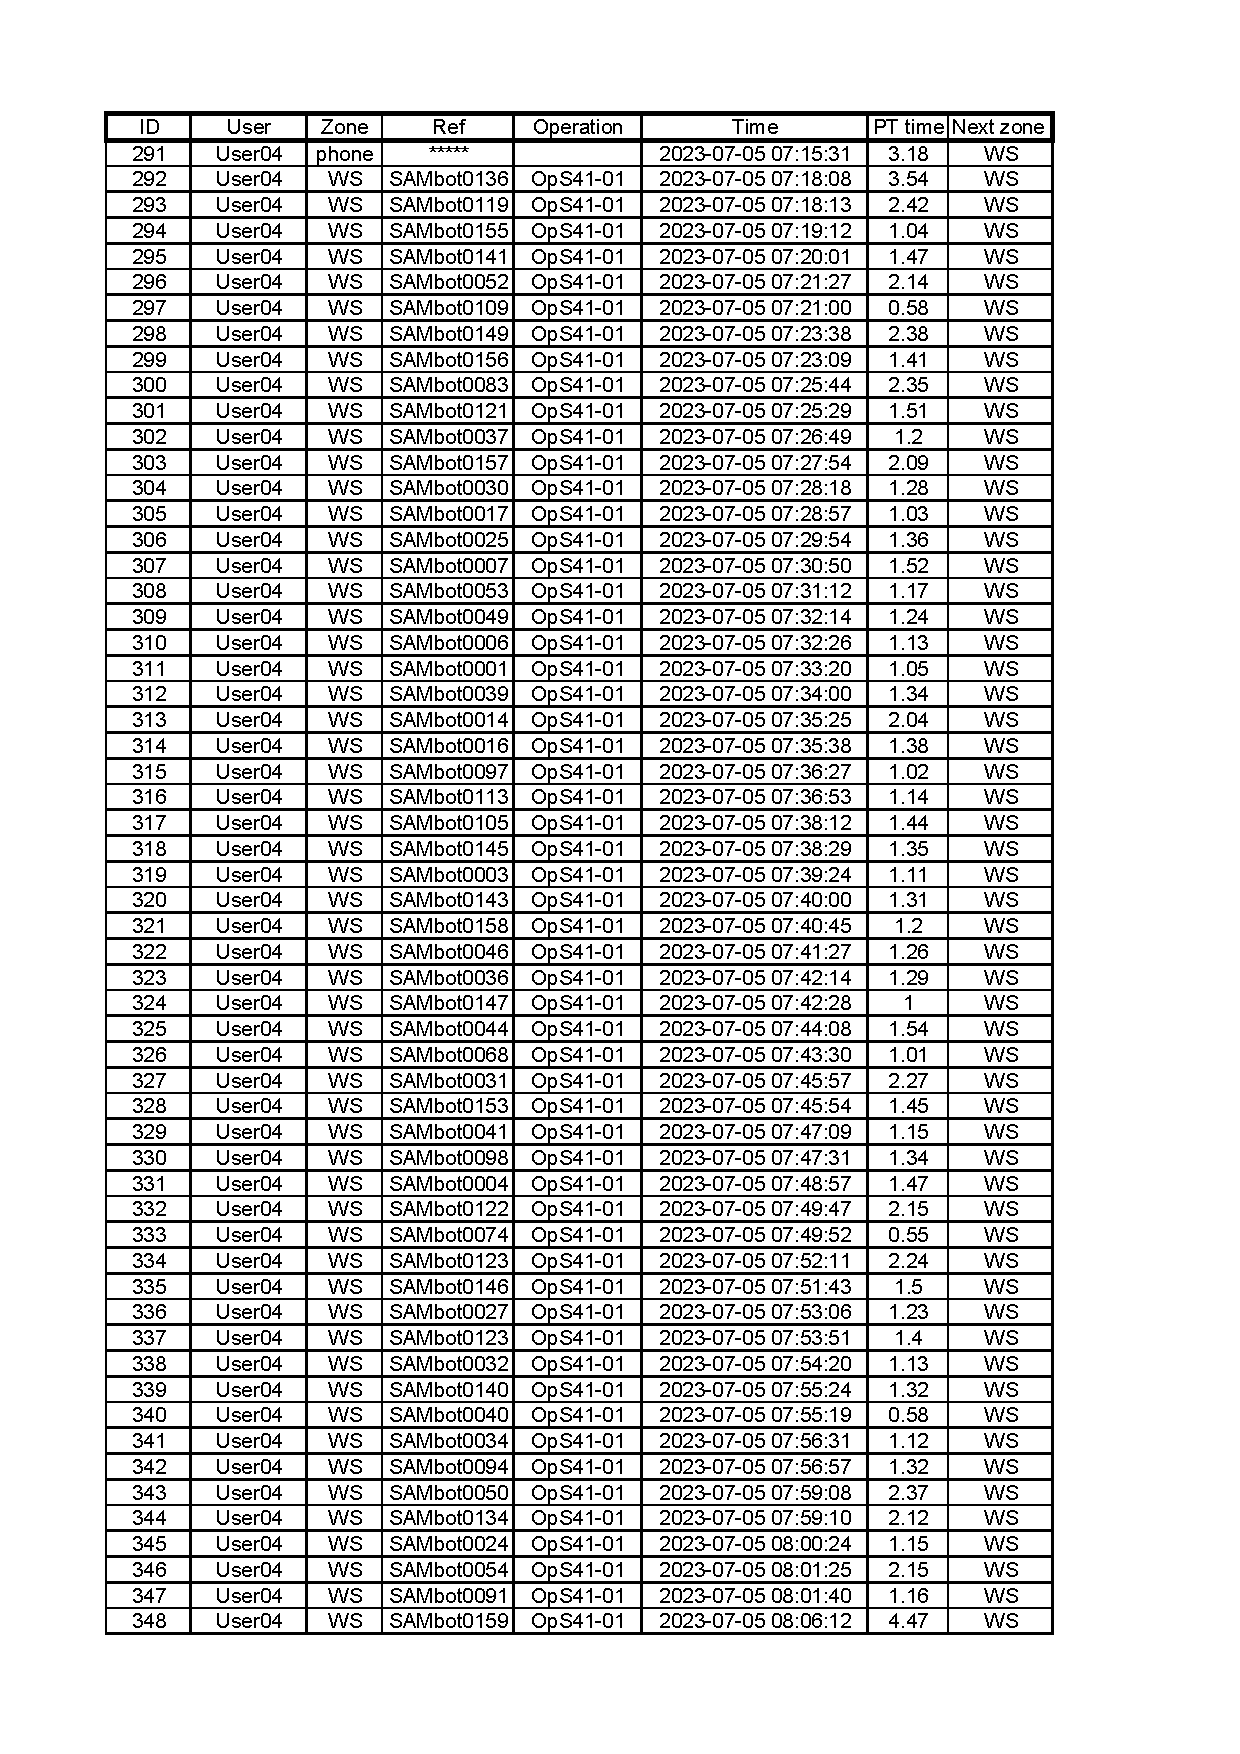
\includepdf[pages=-]{data.pdf}

\end{document}


     


% R1 Q17 G
% R1 Q15 G
% R1 Q19 G
% R1 Q20 G